\newpage
\section{Simulation Analysis}
\label{sec:simulation}

%---------------Simulation Analysis Exercise 1--------------------------------------------------------%
\subsection{Exercise 1}
\label{Simulation Exercise 1}

In this section we proceed to do the anlysis of the circuit through the use of the Ngspice simulation program. In figure~\ref{fig:circuit_simulation} we have the circuit that was inputed into Ngspice (and also the considered current flows and nodes). The file can be found at the $sim$ folder inside the $T2$ folder.

\begin{figure}[!ht] \centering
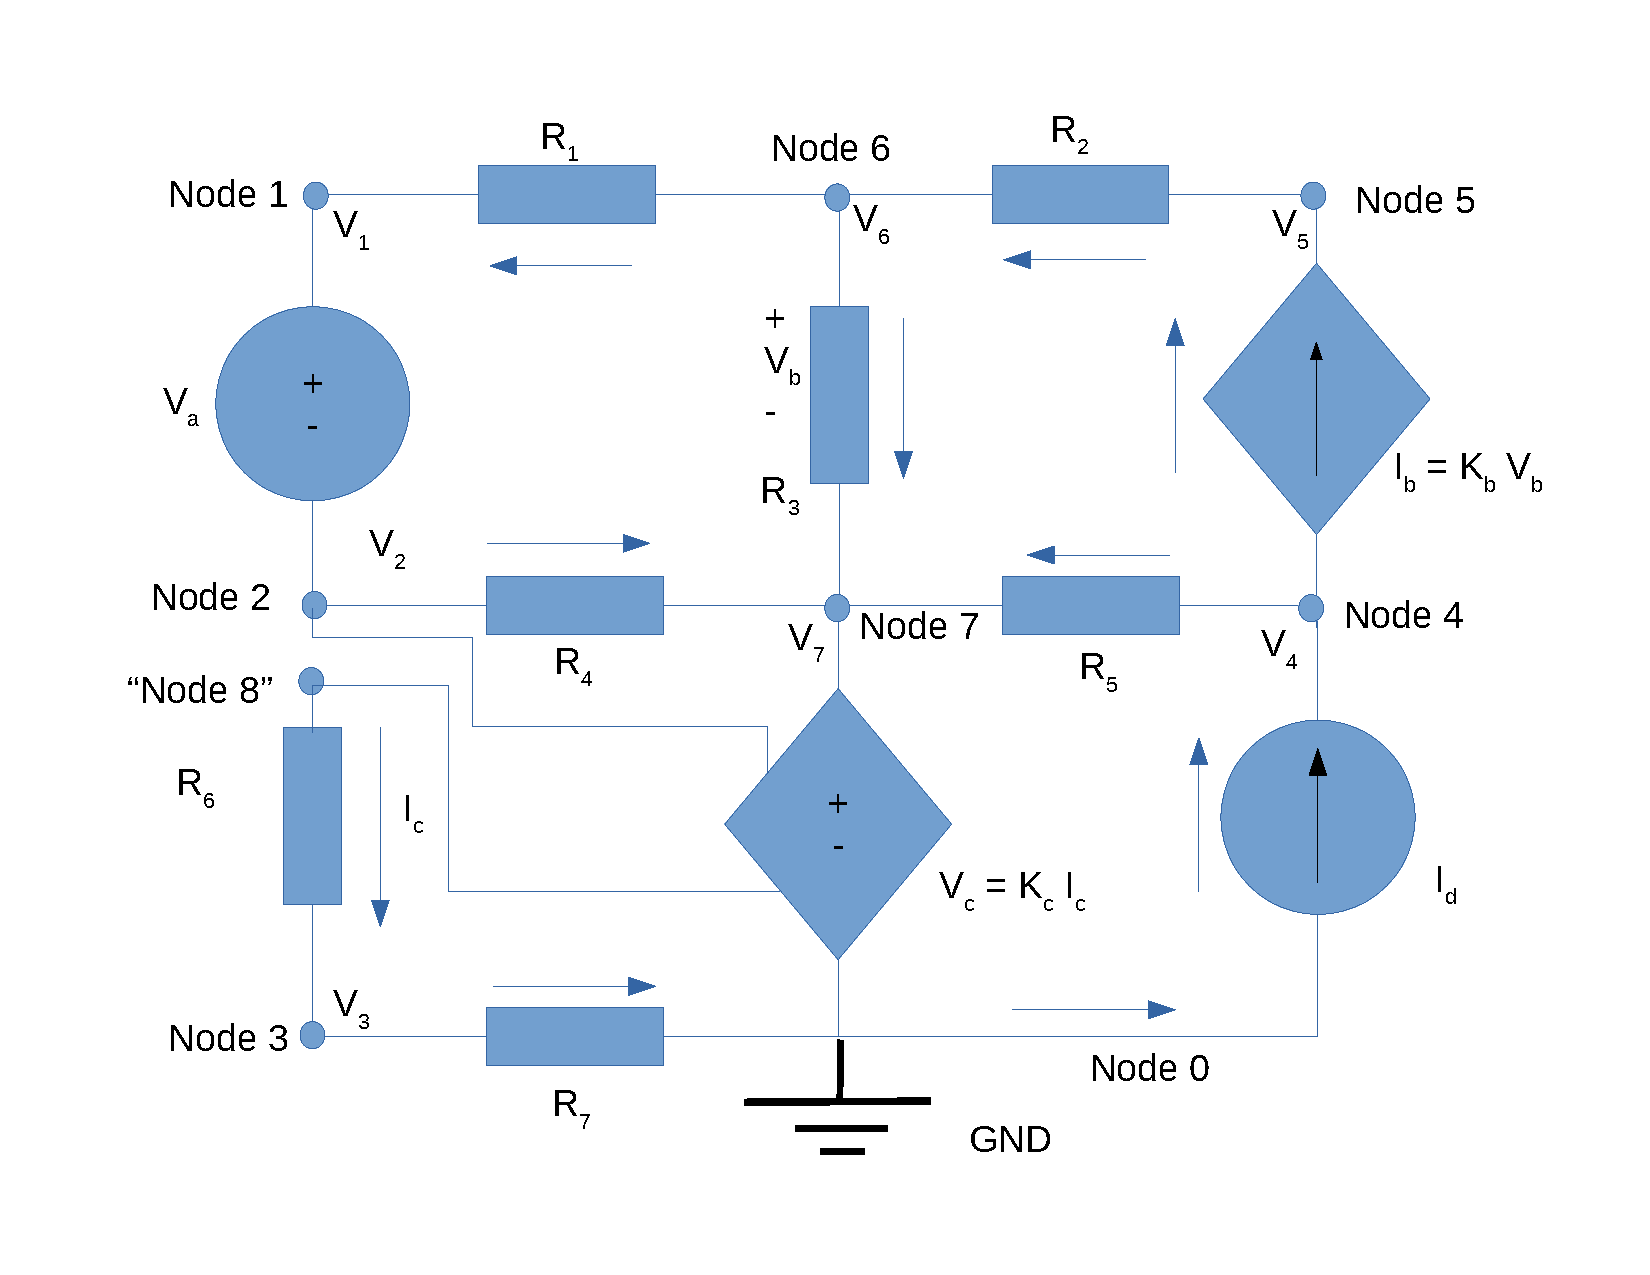
\includegraphics[width=0.8\linewidth]{circuit_simulation.pdf}
\caption{Considered circuit for Ngspice simulation}
\label{fig:circuit_simulation}
\end{figure}

$V_9$ refers to an extra ficticious node created specifically for the Ngspice simulation, and it is below $0(GND)$ and above resistor R6 as it can be seen above in figure~\ref{fig:circuit_simulation}.The reason this node is necessary is because when creating a current controlled voltage source, Ngspice gets the current value by refering to a voltage source from where the current goes through. Since $I_d$ does not go through any voltage source in the circuit (does not go through $V_s$) we used this extra node to create a voltage source of 0$V$ (Which can be confirmed since $V_9 = $GND$ = 0$) from which we are certain $I_d$ is passing by. 

Table~\ref{tab:op} shows the simulated operating point results for the circuit under analysis given the values found on Table~\ref{tab:op1}, considering t<0, which means $v_S(t)$ = $V_s$ as seen in Figure~\ref{fig:circuit}. The variables representation and format are automatically determined by Ngspice.

\begin{table}[!ht]
  \centering
  \caption{Operating point for $t<0$. A variable preceded by @ is of type {\em current}
    and expressed in Ampere; other variables are of type {\it voltage} and expressed in
    Volt. (the g in "gib" refers to the Ngspice notation of a voltage controlled current source)}
  \begin{tabular}{|l|r|}
    \hline    
    {\bf Name} & {\bf Value [A or V]} \\ \hline
    @c1[i] & 0.000000e+00\\ \hline
@gib[i] & -2.45467e-04\\ \hline
@r1[i] & 2.344922e-04\\ \hline
@r2[i] & 2.454667e-04\\ \hline
@r3[i] & 1.097445e-05\\ \hline
@r4[i] & 1.220071e-03\\ \hline
@r5[i] & 2.454667e-04\\ \hline
@r6[i] & 9.855785e-04\\ \hline
@r7[i] & 9.855785e-04\\ \hline
v1 & 5.242048e+00\\ \hline
v2 & 5.002985e+00\\ \hline
v3 & 4.499645e+00\\ \hline
v5 & 5.036927e+00\\ \hline
v6 & 5.789615e+00\\ \hline
v7 & -1.98352e+00\\ \hline
v8 & -2.97405e+00\\ \hline
v9 & 0.000000e+00\\ \hline

  \end{tabular}
  \label{tab:op}
\end{table}

We can get all the missing values given the voltage different of the nodes where they are defined.

\begin{equation}
  V_b = \partialinput{49}{49}{ngspice.log1} V
\end{equation}

\begin{equation}
 V_d = \partialinput{50}{50}{ngspice.log1} V
\end{equation}

%---------------Simulation Analysis Exercise 2--------------------------------------------------------%
\subsection{Exercise 2}
\label{Simulation Exercise 2}
In this section, we simulate the operating point for $v_s(0) = 0$, replacing the capacitor with a voltage source $V_x = V_6 - V_8$ using the values of the respective nodes as obtained in section \ref{Simulation Exercise 1}.

It is required to replace the capacitor since we can assume that an infinite time as passed until t=0 and it is fully charged, meaning it starts with the voltage given before we start the time.

Table~\ref{tab:op2} shows the simulated operating point results for the circuit under analysis given the values found on Table~\ref{tab:op1}, considering t=0, and the above mentioned considerations.

\begin{table}[!ht]
  \centering
  \caption{Operating point for $t = 0$, $v_s(0) = 0$ and capacitor replaced with $V_x = V_6 - V_8$. A variable preceded by @ is of type {\em current}
    and expressed in Ampere; other variables are of type {\it voltage} and expressed in
    Volt. (the g in "gib" refers to the Ngspice notation of a voltage controlled current source)}
  \begin{tabular}{|l|r|}
    \hline    
    {\bf Name} & {\bf Value [A or V]} \\ \hline
    @gib[i] & 0.000000e+00\\ \hline
@r1[i] & 0.000000e+00\\ \hline
@r2[i] & 0.000000e+00\\ \hline
@r3[i] & 0.000000e+00\\ \hline
@r4[i] & 0.000000e+00\\ \hline
@r5[i] & 2.858009e-03\\ \hline
@r6[i] & 0.000000e+00\\ \hline
@r7[i] & 0.000000e+00\\ \hline
v1 & 0.000000e+00\\ \hline
v2 & 0.000000e+00\\ \hline
v3 & 0.000000e+00\\ \hline
v5 & 0.000000e+00\\ \hline
v6 & 8.763669e+00\\ \hline
v7 & 0.000000e+00\\ \hline
v8 & 0.000000e+00\\ \hline
v9 & 0.000000e+00\\ \hline
v(v5,v2) & 0.000000e+00\\ \hline
v(v8,v5) & 0.000000e+00\\ \hline

  \end{tabular}
  \label{tab:op2}
\end{table}

%---------------Simulation Analysis Exercise 3--------------------------------------------------------%
\subsection{Exercise 3}
\label{Simulation Exercise 3}
In this section we used the results obtained in section \ref{Simulation Exercise 2} to determine the natural solution $v_{6n}(t)$ in the interval $[0,20]ms$ using the boundary conditions $V_6$ and $V_8$.

Figure ~\ref{fig:simulation_3} shows the plot of the required result that was obtained using the transient analysis.

\begin{figure}[!ht] \centering
\caption{Natural solution, $v_{6n}(t)$ in $V$ in the interval $[0,20]ms$}
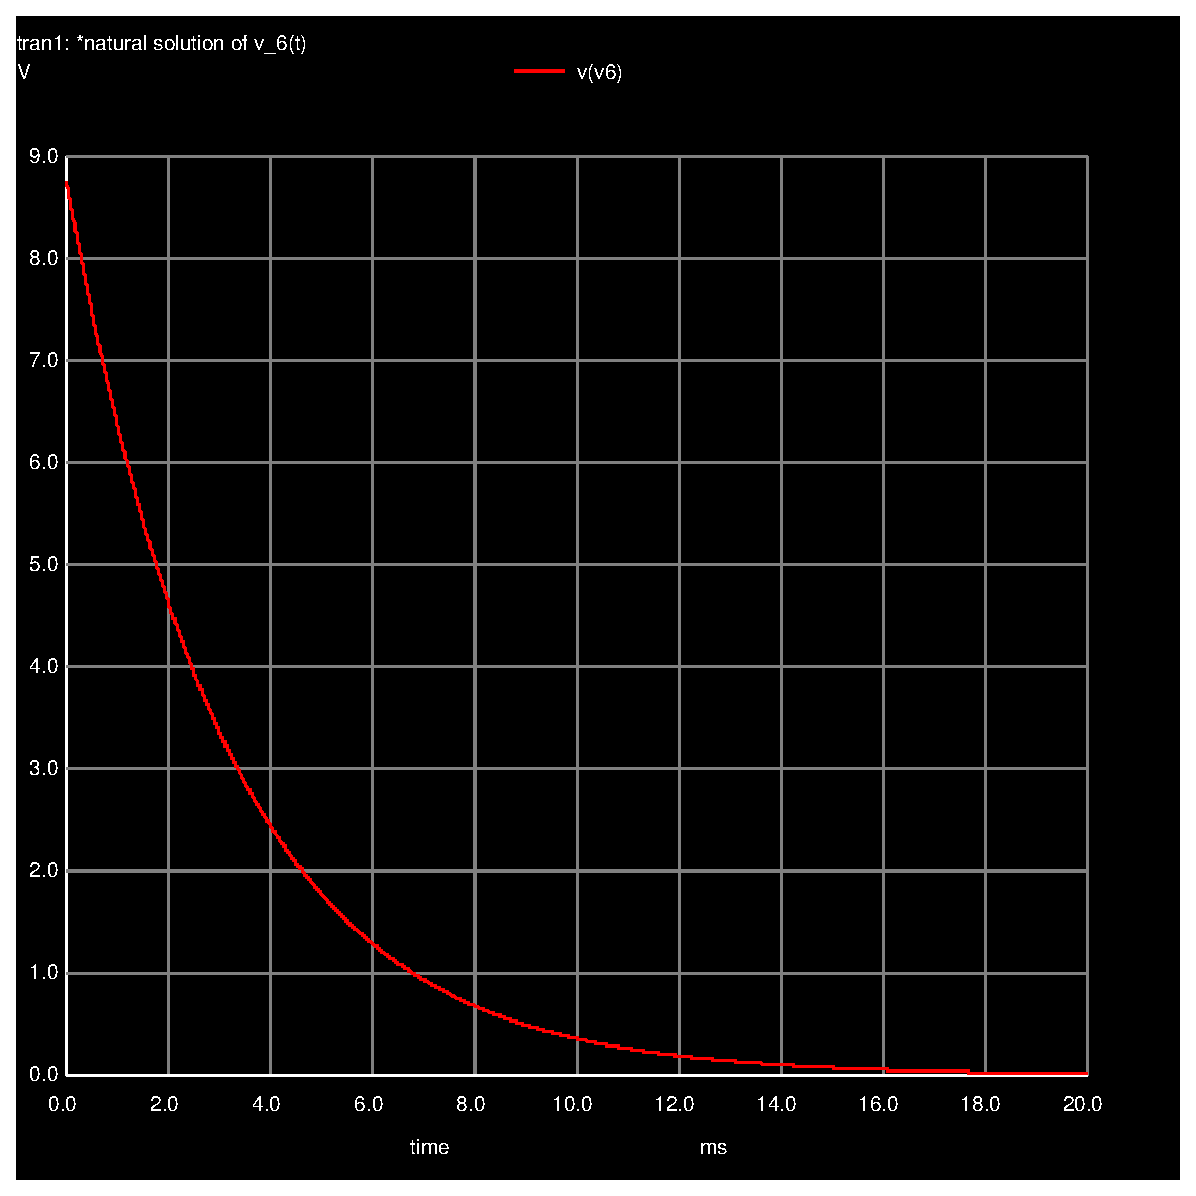
\includegraphics[width=0.8\linewidth]{trans3.eps}
\label{fig:simulation_3}
\end{figure}

%---------------Simulation Analysis Exercise 4--------------------------------------------------------%
\subsection{Exercise 4}
\label{Simulation Exercise 4}
In this section we are required to simulate the total response in node 6 $v_{6}(t)$ by repeating the procedure of \ref{Simulation Exercise 3} with the initially given $v_s(t)$ (shown in \ref{fig:circuit}, with a frequency of $1000 Hz$.

Figure ~\ref{fig:simulation_4} shows the plot of the required result that was obtained using the transient analysis as well as the stimulus (shown as $v(V_1)$ since $v_1(t) = v_s(t)$

\begin{figure}[!ht] \centering
\caption{Total response, $v_{6}(t)$ in $V$, and stimulus $v_s(t)$, in $V$ in the interval $[0,20]ms$}
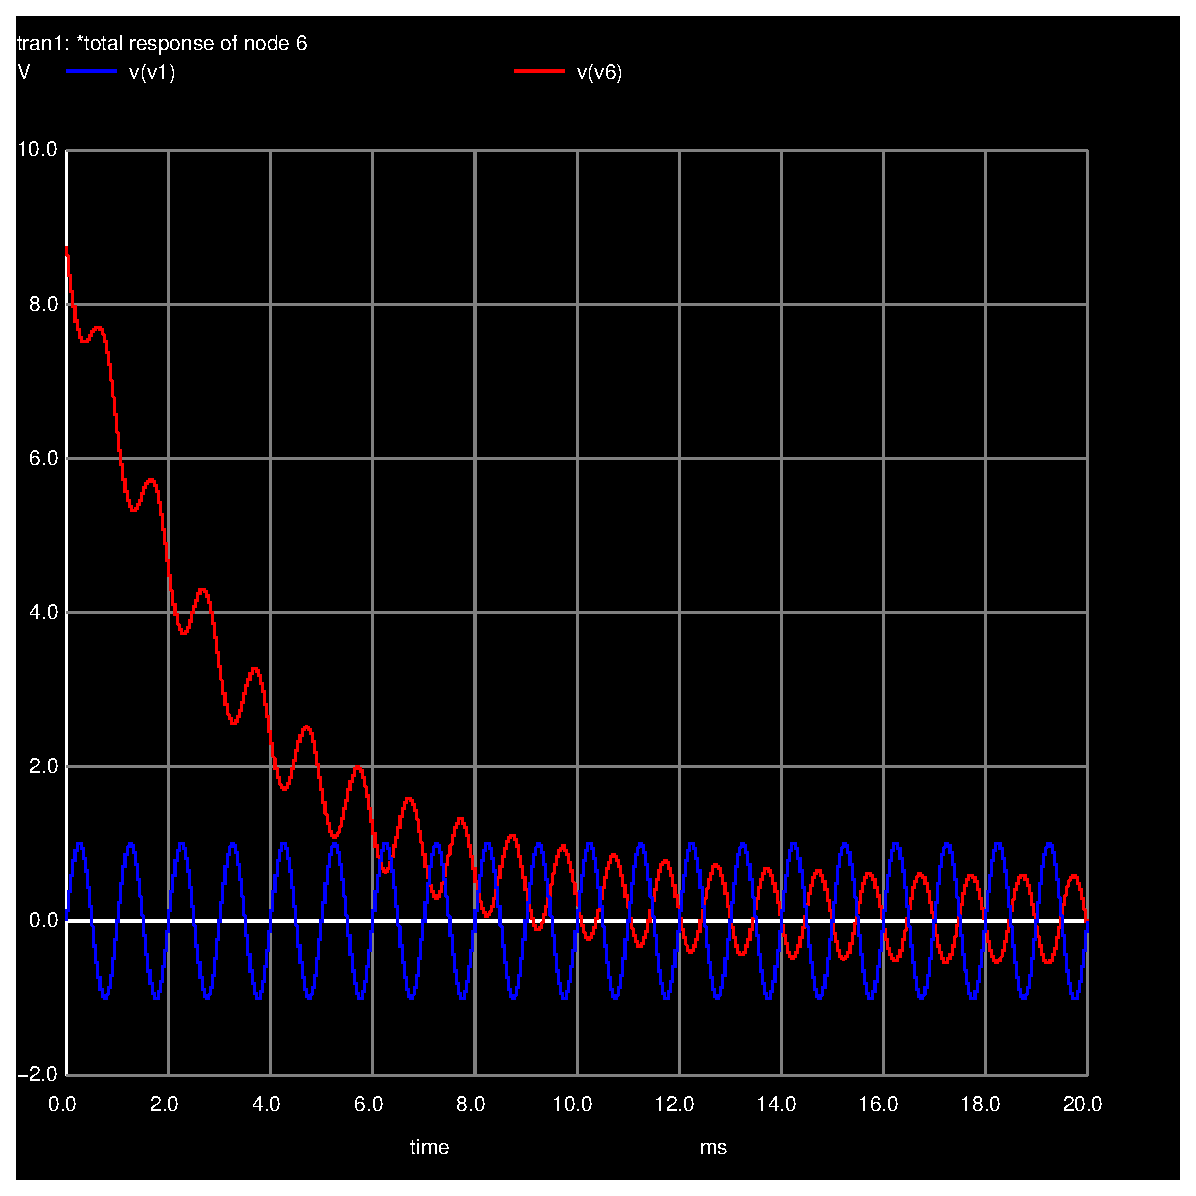
\includegraphics[width=0.8\linewidth]{trans4.eps}
\label{fig:simulation_4}
\end{figure}


%---------------Simulation Analysis Exercise 5--------------------------------------------------------%
\newpage
\subsection{Exercise 5}
\label{Simulation Exercise 5}
In this section we are required to simulate the frequency response in node 6 $v_{6}(t)$ with the frequency in logscale, magnitude in $dB$ and phase in degrees for a range of $0.1Hz$ to $1MHz$.

Figure ~\ref{fig:simulation_5} shows the plot of the required result, $v_6(f)$ as well as $v_s(f)$.

\begin{figure}[!ht] \centering
\caption{Frequency response, $v_{6}(f)$ in $V$, and $v_s(f)$, in $V$. Phase is in degrees and Magnitude in $dB$}
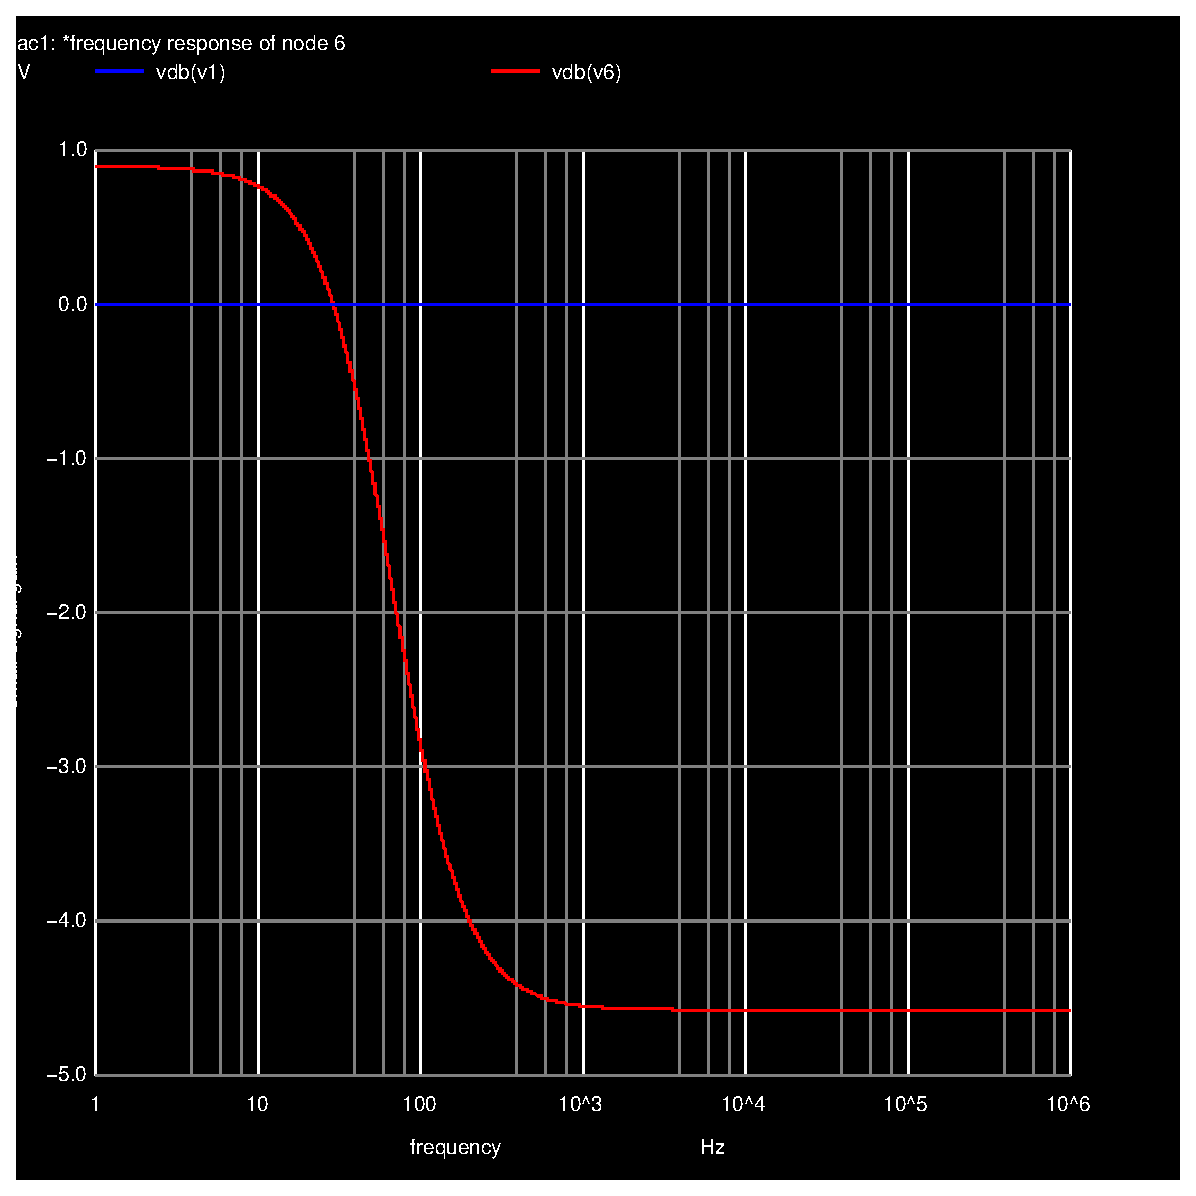
\includegraphics[width=0.4\linewidth]{acm.eps}
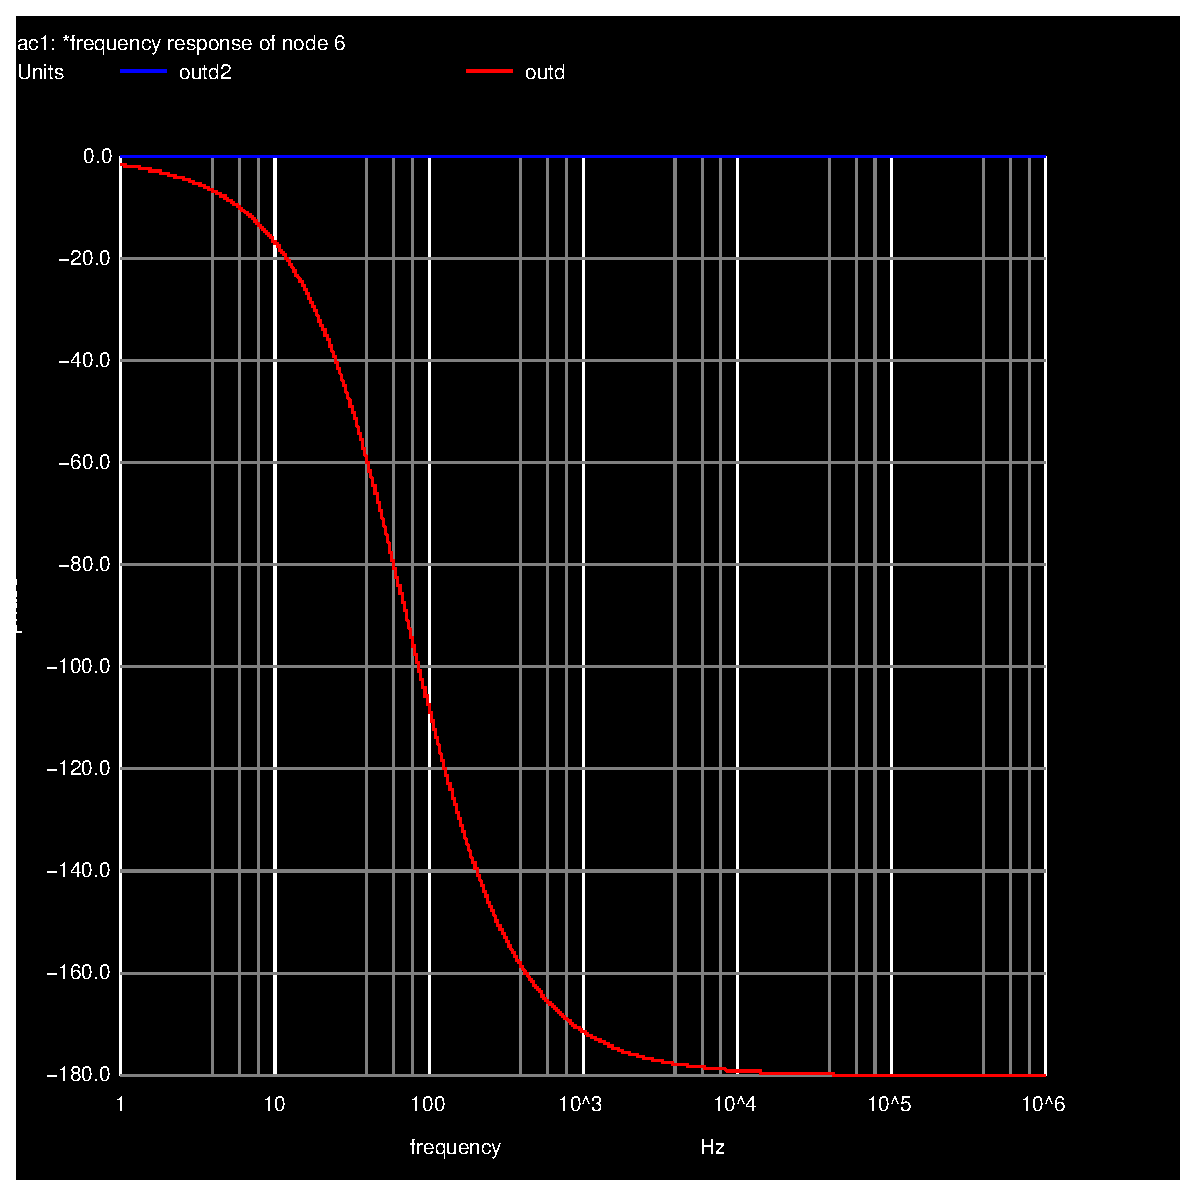
\includegraphics[width=0.4\linewidth]{acm2.eps}
\label{fig:simulation_5}
\end{figure}

Since the source of of frequency change is $v_s$ itself, it is expected to not to show a frequency response since it changes alongside frequency, where as $v_6$ is dependant of the value that $v_s$ takes. 







